\documentclass{beamer}

% Should be documentclass beamer

\mode<presentation>
{
%  \usetheme[hideothersubsections]{PaloAlto}
  \usetheme{metropolis}
  \setbeamercovered{transparent}
}

\usepackage{amsfonts}
\usepackage{amsmath}
\usepackage{amssymb}
\usepackage{color}
\usepackage{tikz}
\usepackage{pgfplots}
\usepackage{listings}
\usepackage{courier}
%\usepackage[utf8]{inputenc}
%\usepackage[russian]{babel}

\lstset{
  numbers=left,
  basicstyle=\ttfamily\footnotesize,
  numberstyle=\tiny\color{gray},
  stepnumber=1,
  numbersep=10pt,
}

\newcommand{\iu}{\ensuremath{\mathrm{i}}}
\newcommand{\bbR}{\mathbb{R}}
\newcommand{\bbC}{\mathbb{C}}
\newcommand{\calV}{\mathcal{V}}
\newcommand{\calW}{\mathcal{W}}
\newcommand{\macheps}{\epsilon_{\mathrm{mach}}}
\newcommand{\matlab}{\textsc{Matlab}}

\newcommand{\ddiag}{\operatorname{diag}}
\newcommand{\fl}{\operatorname{fl}}
\newcommand{\nnz}{\operatorname{nnz}}
\newcommand{\tr}{\operatorname{tr}}
\renewcommand{\vec}{\operatorname{vec}}

\newcommand{\vertiii}[1]{{\left\vert\kern-0.25ex\left\vert\kern-0.25ex\left\vert #1
    \right\vert\kern-0.25ex\right\vert\kern-0.25ex\right\vert}}
\newcommand{\ip}[2]{\langle #1, #2 \rangle}
\newcommand{\ipx}[2]{\left\langle #1, #2 \right\rangle}
\newcommand{\order}[1]{O( #1 )}

\newcommand{\kron}{\otimes}


\newcommand{\hdr}[2]{
  \title[CS 5220, Fall 2017]{CS 5220: #2}
  \author{David Bindel}
  \date{#1}
}

\hdr{2017-08-29}{Single core architecture}

\begin{document}


\begin{frame}
  \titlepage
\end{frame}


\begin{frame}
  \frametitle{Just for fun}
  
  \begin{center}
  \url{http://www.youtube.com/watch?v=fKK933KK6Gg}
  \end{center}

  \begin{center}
    Is this a fair portrayal of your CPU? \\[5mm]
    (See Rich Vuduc's talk, 
    \href{http://web.eecs.utk.edu/~dongarra/ccgsc2010/slides/talk27-vuduc.pdf}
         {``Should I port my code to a GPU?''})
  \end{center}
\end{frame}

\begin{frame}
  \frametitle{The idealized machine}
  
  \begin{center}
%    \includegraphics[width=0.4\textwidth]{smiley.pdf}
  \end{center}

  \begin{itemize}
  \item Address space of named words
  \item Basic operations are register read/write, logic, arithmetic
  \item Everything runs in the program order
  \item High-level language $\rightarrow$ ``obvious'' machine code
  \item All operations take about the same amount of time
  \end{itemize}
\end{frame}

\begin{frame}
  \frametitle{The real world}

  \begin{center}
%    \includegraphics[width=0.22\textwidth]{monalisa.jpg}
  \end{center}

  \begin{itemize}
  \item Memory operations are {\em not} all the same!
    \begin{itemize}
    \item Registers and caches lead to variable access speeds
    \item Different memory layouts dramatically affect performance
    \end{itemize}
  \item Instructions are non-obvious!
    \begin{itemize}
    \item Pipelining allows instructions to overlap
    \item Functional units run in parallel (and out of order)
    \item Instructions take different amounts of time
    \item Different costs for different orders and instruction mixes
    \end{itemize}
  \end{itemize}

  Our goal: enough understanding to help the compiler out.
\end{frame}

\begin{frame}
  \frametitle{Prelude}

  We hold these truths to be self-evident:
  \begin{enumerate}
  \item One should not sacrifice correctness for speed
  \item One should not re-invent (or re-tune) the wheel
  \item Your time matters more than computer time
  \end{enumerate}
  
  Less obvious, but still true:
  \begin{enumerate}
  \item Most of the time goes to a few bottlenecks
  \item The bottlenecks are hard to find without measuring
  \item Communication is expensive (and often a bottleneck)
  \item A little good hygiene will save your sanity
    \begin{itemize}
    \item Automate testing, time carefully, and use version control
    \end{itemize}
  \end{enumerate}
\end{frame}

\begin{frame}
  \frametitle{A sketch of reality}

  Today, a play in two acts:%
\footnote{%
If you don't get the reference to {\em This American Life},
go find the podcast!}
  \begin{enumerate}
  \item Act 1: One core is not so serial
  \item Act 2: Memory matters
  \end{enumerate}
\end{frame}

\begin{frame}
  \frametitle{Act 1}
  One core is not so serial.
\end{frame}

\begin{frame}
  \frametitle{Parallel processing at the laundromat}

  \begin{itemize}
  \item Three stages to laundry: wash, dry, fold.
  \item Three loads: {\color{blue} darks}, {\color{red} lights}, {\color{green} underwear}
  \item How long will this take?
  \end{itemize}
\end{frame}

\begin{frame}
  \frametitle{Parallel processing at the laundromat}

  \begin{itemize}
  \item Serial version: \\[2mm]
        \begin{tabular}{lllllllll}
          1 & 2 & 3 & 4 & 5 & 6 & 7 & 8 & 9 \\ \hline
          {\color{blue} wash} & {\color{blue} dry} & {\color{blue} fold} & & & & & & \\
          & & & {\color{red} wash} & {\color{red} dry} & {\color{red} fold} & & & \\
          & & & & & & {\color{green} wash} & {\color{green} dry} & {\color{green} fold} \\ \hline
        \end{tabular}
  \item Pipeline version: \\[2mm]
        \begin{tabular}{lllll|l}
          1 & 2 & 3 & 4 & 5 \\ \hline
          {\color{blue} wash} & {\color{blue} dry} & {\color{blue} fold} & & & Dinner? \\
          & {\color{red} wash} & {\color{red} dry} & {\color{red} fold} & & Cat videos? \\
          & & {\color{green} wash} & {\color{green} dry} & {\color{green} fold} & Gym and tanning? \\ \hline
        \end{tabular}

  \end{itemize}
\end{frame}

\begin{frame}
  \frametitle{Pipelining}
  
  \begin{itemize}
  \item Pipelining improves {\em bandwidth}, but not {\em latency}
  \item Potential speedup = number of stages
    \begin{itemize}
    \item But what if there's a branch?
    \end{itemize}
  \item Different pipelines for different functional units
    \begin{itemize}
    \item Front-end has a pipeline
    \item Functional units (FP adder, FP multiplier) pipelined
    \item Divider is frequently not pipelined
    \end{itemize}
  \end{itemize}
\end{frame}


% TODO:
% Reference to more complications: out-of-order execution engines,
% micro-instructions.  Compiler helps.  Key issue: dependencies.

\begin{frame}
  \frametitle{Out-of-order execution}

  Modern CPUs are {\em wide} and {\em out-of-order}:
  \begin{itemize}
  \item Wide: Fetch/decode or retire multiple ops at once
    \begin{itemize}
    \item Limits: Instruction mix (different ports for different ops)
    \item NB: May dynamically translate to micro-ops
    \end{itemize}
  \item Out-of-order: {\em Looks} in-order, internally not!
    \begin{itemize}
    \item Limits: Data dependencies
    \end{itemize}
  \item Details are {\em very} hard to work out manually
    \begin{itemize}
    \item Don't generally know the micro-op breakdown!
    \item Tricky to think through even if we did
    \item Compilers help a lot with this
    \item But they need a good mix of independent ops
    \end{itemize}
  \end{itemize}
\end{frame}


\begin{frame}
  \frametitle{SIMD}

  \begin{itemize}
  \item {\em S}ingle {\em I}nstruction {\em M}ultiple {\em D}ata
  \item Cray-1 (1976): 8 registers $\times$ 64 words of 64 bits each
  \item Old idea had a resurgence in mid-late 90s (for graphics)
  \item Now short vectors are ubiquitous...
    \begin{itemize}
    \item Totient CPUs: 256 bits (four doubles) in a vector (AVX)
    \item Totient accel: 512 bits (eight doubles) in a vector (AVX-512)
    \item And then there are GPUs!
    \end{itemize}
  \item Alignment often matters
  \end{itemize}
\end{frame}


\begin{frame}
  \frametitle{Example: My laptop}

  \href{http://ark.intel.com/products/75991/Intel-Core-i5-4288U-Processor-3M-Cache-up-to-3_10-GHz}{MacBook Pro (Retina, 13 in, late 2013).}
  \begin{itemize}
  \item Intel Core i5-4288U CPU at 2.6 GHz.  2 core / 4 thread.
  \item AVX units provide up to 8 double flops/cycle \\
        (Simultaneous vector add + vector multiply)
  \item Wide dynamic execution: up to four full instructions at once
    \begin{itemize}
    \item Haswell has two FMA ports, so can retire two at a time
    \end{itemize}
  \item Operations internally broken down into ``micro-ops''
    \begin{itemize}
    \item Cache micro-ops -- like a hardware JIT?!
    \end{itemize}
  \end{itemize}
  Theoretical peak: 83.2 GFlop/s?

\end{frame}

\begin{frame}
  \frametitle{Punchline}
  
  \begin{itemize}
  \item Special features: SIMD instructions, maybe FMAs, ...
  \item Compiler understands how to utilize these {\em in principle}
    \begin{itemize}
    \item Rearranges instructions to get a good mix
    \item Tries to make use of FMAs, SIMD instructions, etc
    \end{itemize}
  \item In practice, needs some help:
    \begin{itemize}
    \item Set optimization flags, pragmas, etc
    \item Rearrange code to make things obvious and predictable
    \item Use special intrinsics or library routines
    \item Choose data layouts, algorithms that suit the machine
    \end{itemize}
  \item Goal: You handle high-level, compiler handles low-level.
  \end{itemize}
    
\end{frame}

\begin{frame}
  \frametitle{Act 2}
  Memory matters.
\end{frame}


\begin{frame}
  \frametitle{My machine}

  \begin{itemize}
  \item Theoretical peak flop rate: 83.2 GFlop/s
  \item Peak memory bandwidth: 25.6 GB/s
  \item Arithmetic intensity = flops / memory accesses
  \item Example: Sum several million doubles (AI = 1) -- how fast?
  \item So what can we do?  Not much if lots of fetches, but...
  \end{itemize}
\end{frame}


\begin{frame}
  \frametitle{Cache basics}
  
  Programs usually have {\em locality}
  \begin{itemize}
  \item {\em Spatial locality}: things close to each other tend to be
    accessed consecutively
  \item {\em Temporal locality}: use a ``working set'' of data repeatedly
  \end{itemize}
  Cache hierarchy built to use locality.

\end{frame}


\begin{frame}
  \frametitle{Cache basics}

  \begin{itemize}
  \item Memory {\em latency} = how long to get a requested item
  \item Memory {\em bandwidth} = how fast memory can provide data
  \item Bandwidth improving faster than latency
  \end{itemize}

  Caches help:
  \begin{itemize}
  \item Hide memory costs by reusing data
    \begin{itemize}
    \item Exploit temporal locality
    \end{itemize}
  \item Use bandwidth to fetch a {\em cache line} all at once
    \begin{itemize}
    \item Exploit spatial locality
    \end{itemize}
  \item Use bandwidth to support multiple outstanding reads
  \item Overlap computation and communication with memory
    \begin{itemize}
    \item Prefetching
    \end{itemize}
  \end{itemize}

  This is mostly automatic and implicit.

\end{frame}


\begin{frame}
  \frametitle{Cache basics}

  \begin{itemize}
  \item Store cache {\em line}s of several bytes
  \item Cache {\em hit} when copy of needed data in cache
  \item Cache {\em miss} otherwise.  Three basic types:
    \begin{itemize}
    \item {\em Compulsory} miss: never used this data before
    \item {\em Capacity} miss: filled the cache with other things
      since this was last used -- working set too big
    \item {\em Conflict} miss: insufficient associativity for access
      pattern
    \end{itemize}
    \item {\em Associativity}
      \begin{itemize}
      \item Direct-mapped: each address can only go in one cache location
        (e.g. store address xxxx1101 only at cache location 1101)
      \item $n$-way: each address can go into one of $n$ possible cache
        locations (store up to 16 words with addresses xxxx1101 at cache
        location 1101).
      \end{itemize}
      Higher associativity is more expensive.
  \end{itemize}

\end{frame}


\begin{frame}
  \frametitle{Teaser}

  We have $N = 10^6$ two-dimensional coordinates, and want their centroid.
  Which of these is faster and why?
  \begin{enumerate}
  \item
    Store an array of $(x_i, y_i)$ coordinates.  Loop $i$ and simultaneously
    sum the $x_i$ and the $y_i$.
  \item
    Store an array of $(x_i, y_i)$ coordinates.  Loop $i$ and sum the $x_i$,
    then sum the $y_i$ in a separate loop.
  \item
    Store the $x_i$ in one array, the $y_i$ in a second array.  Sum the
    $x_i$, then sum the $y_i$.
  \end{enumerate}
  Let's see!

\end{frame}


\begin{frame}
  \frametitle{Caches on my laptop (I think)}

  \begin{itemize}
  \item 32 KB L1 data and memory caches (per core), \\
    8-way associative
  \item 256 KB L2 cache (per core), \\
    8-way associative
  \item 3 MB L3 cache (shared by all cores)
  \end{itemize}
\end{frame}


\begin{frame}[fragile]
  \frametitle{A memory benchmark (membench)}

\begin{verbatim}
  for array A of length L from 4 KB to 8MB by 2x
    for stride s from 4 bytes to L/2 by 2x
    time the following loop
      for i = 0 to L by s
        load A[i] from memory
\end{verbatim}

\end{frame}


\begin{frame}
  \frametitle{membench on my laptop -- what do you see?}

  \begin{center}
    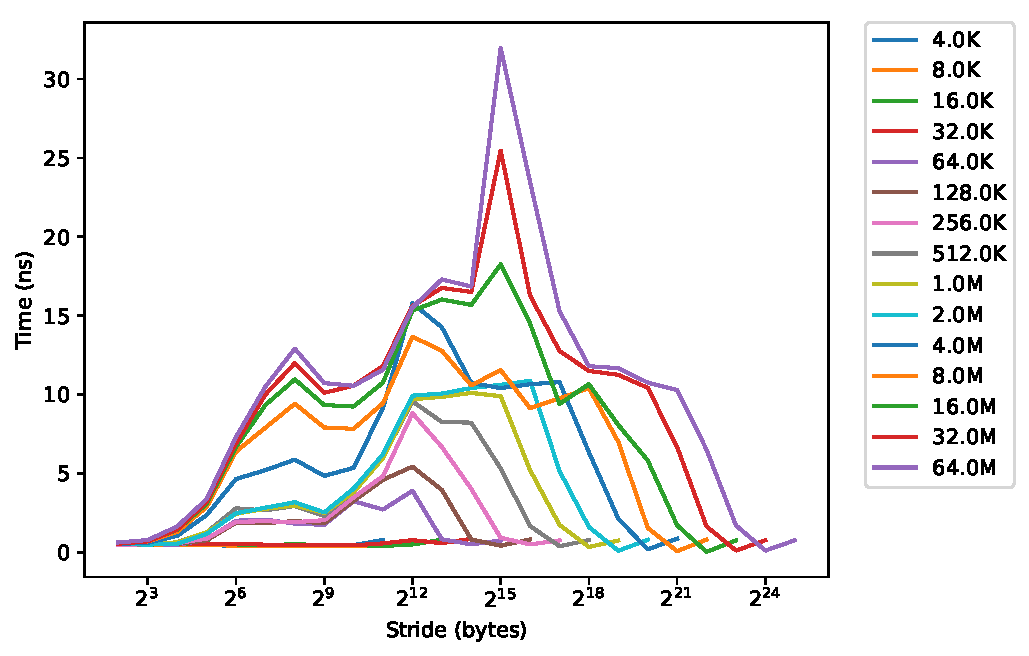
\includegraphics[width=\textwidth]{figs/membench/timings_laptop-line.pdf}
  \end{center}
\end{frame}


\begin{frame}
  \frametitle{membench on my laptop -- what do you see?}

  \begin{center}
    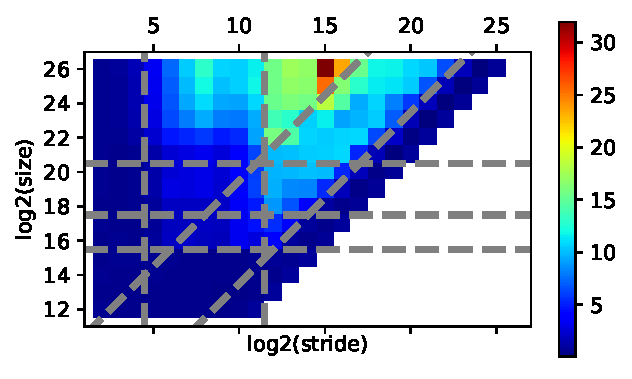
\includegraphics[width=\textwidth]{figs/membench/timings_laptop-heat.pdf}
  \end{center}
\end{frame}


\begin{frame}
  \frametitle{membench on my laptop -- what do you see?}

  \begin{center}
    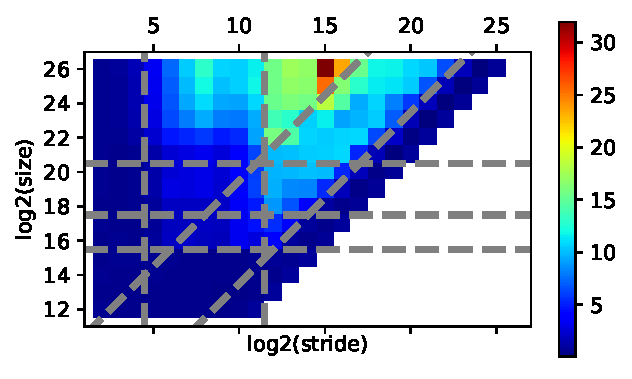
\includegraphics[width=0.75\textwidth]{figs/membench/timings_laptop-heat.pdf}
  \end{center}
  \begin{itemize}
    \item Vertical: 64B line size ($2^5$), 4K page size ($2^{12}$)
    \item Horizontal: 32K L1 ($2^{15}$), 256K L2 ($2^{18}$), 6 MB L3
    \item Diagonal: 8-way cache associativity, 512 entry L2 TLB
  \end{itemize}
\end{frame}


\begin{frame}
    \frametitle{membench on Totient -- what do you see?}

  \begin{center}
    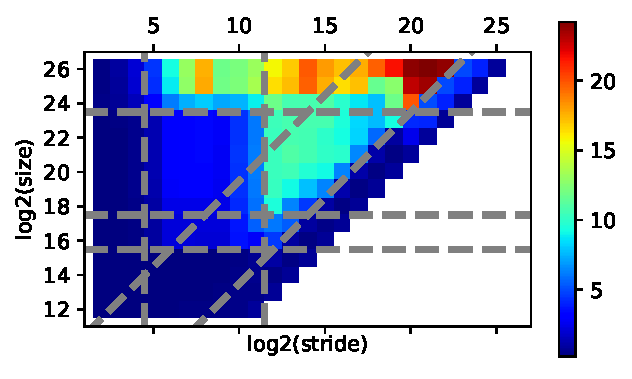
\includegraphics[width=\textwidth]{figs/membench/timings_totient-heat.pdf}
  \end{center}
\end{frame}


\begin{frame}
  \frametitle{The moral}
  
  Even for simple programs, performance is a complicated function of
  architecture!
  \begin{itemize}
  \item Need to understand at least a little to write fast programs
  \item Would like simple models to help understand efficiency
  \item Would like common tricks to help design fast codes
    \begin{itemize}
    \item Example: {\em blocking} (also called {\em tiling})
    \end{itemize}
  \end{itemize}
\end{frame}


\begin{frame}
  \frametitle{Coda}
  The Roofline Model.
\end{frame}


\begin{frame}
  \frametitle{Roofline model}

  S. Williams, A. Waterman, D. Patterson,
  ``\href{http://www.eecs.berkeley.edu/Pubs/TechRpts/2008/EECS-2008-134.pdf}{Roofline:
    An Insightful Visual Performance Model for Floating-Point Programs
    and Multicore Architectures},'' CACM, April 2009.
\end{frame}


% TODO: Add a few slides on roofline; parameters for Totient and for
% my laptop?

\begin{frame}
  \frametitle{Roofline plot basics}

  Log-log plot (base 2)
  \begin{itemize}
  \item $x$: Operational intensity (flops/byte)
  \item $y$: Attainable performance (GFlop/s)
  \item Diagonals: Memory limits
  \item Horizontals: Compute limits
  \item Papers: \url{https://crd.lbl.gov/departments/computer-science/PAR/research/roofline/}
  \item Tools: \url{https://bitbucket.org/berkeleylab/cs-roofline-toolkit}
  \end{itemize}
\end{frame}


\end{document}
